\section{Experiments}
\seclabel{experiments}

We evaluate the convergence rate of the Dex-Net 1.0 algorithm using force closure as our binary quality metric for varying sizes of prior data used from Dex-Net, and we explore the sensitivity of the convergence rate to object shape, the similarity kernel bandwidths, and uncertainty.
We created two training sets of 1,000, and 10,000 objects by uniformly sampling objects from Dex-Net.
We uniformly sampled a set of 300 validation objects for selecting algorithm hyperparameters and selected a set of 45 test objects from the remaining objects.
We ran the algorithm with $M = 10$ nearest neighbors, $\alpha_0 = \beta_0 = 1$~\cite{laskey2015bandits}, and a lower confidence bound containing $q=75\%$ of the belief distribution.
We used isotropic Gaussian uncertainty with object and gripper translation variance $\sigma_{t} = 0.005$, object and gripper rotation variance $\sigma_{r} = 0.1$, and friction variance $\sigma_{\gamma} = 0.1$.
For each experiment we compare the Dex-Net algorithm to Thompson sampling without priors (TS)~\cite{laskey2015bandits}, a state-of-the-art method for robust grasp planning, and uniform allocation (UA), a widely-used method for robust grasp planning the selects the next grasp to evaluate uniformly at random~\cite{kehoe2012toward, kim2012physically, weisz2012pose}.

The inverse kernel bandwidths were selected by maximizing the log-likelihood of the true $P_F$ under the CCBP model~\cite{goetschalckx2011continuous} on the validation set using a grid search over hyperparameters.
The inverse bandwidths of the similarity kernel were $C_g = diag(0,0,3e-5, 3e-5)$ for the grasp parameter features, an isotropic Gaussian mask $C_d$ with mean $\mu_d = 500.0$ and $\sigma_d = 0.33$ for the differential heightmap features, and $C_s = 1e6 * I$ for the shape similarity features.

To scale experiments, we developed a Cloud-based system on top of Google Cloud Platform.
We used Google Compute Engine (GCE) to construct the Dex-Net 1.0 dataset and to distribute subsets of objects to virtual machines for MAB experiments, and we used Google Cloud Storage to store Dex-Net.
The system launched up to 1,500 GCE virtual instances at once for experiments, reducing the runtime by an estimated three orders of magnitude to approximately 315 seconds per object.
Each virtual instance ran Ubuntu 12.04 on a single core with 3.75 GB of RAM.

\subsection{Scaling of Average Convergence Rate}
\seclabel{conv-rate}
To examine the effects of orders of magnitude of prior data on convergence to a grasp with high $P_F$, we ran the Dex-Net 1.0 algorithm on the test objects with priors computed from 1,000 and 10,000 objects from Dex-Net. 
~\figref{avg-reward} shows the normalized $P_F$  (the ratio of the $P_F$ for the best grasp predicted by the algorithm on iteration $t$ to the highest $P_F$ of the candidate grasps) versus iteration averaged over 25 trials for each of the test objects over 2,000 iterations.
The average runtime per iteration was 16 ms for UA, 17 ms for TS, and 22 ms for Dex-Net 1.0.
The algorithm with 10,000 objects takes approximately 2$\times$ fewer iterations to reach the maximum normalized $P_F$ value reached by TS.
Furthermore, the 10,000 object curve does not fall below approximately 90\% of the best grasp in the set across all iterations, suggesting that a grasp with high $P_F$ is found using prior data alone.
This speedup is promising for binary success metrics that are expensive to  evaluate, such as human labels or physical grasping trials.

\begin{figure}[t!]
\centering
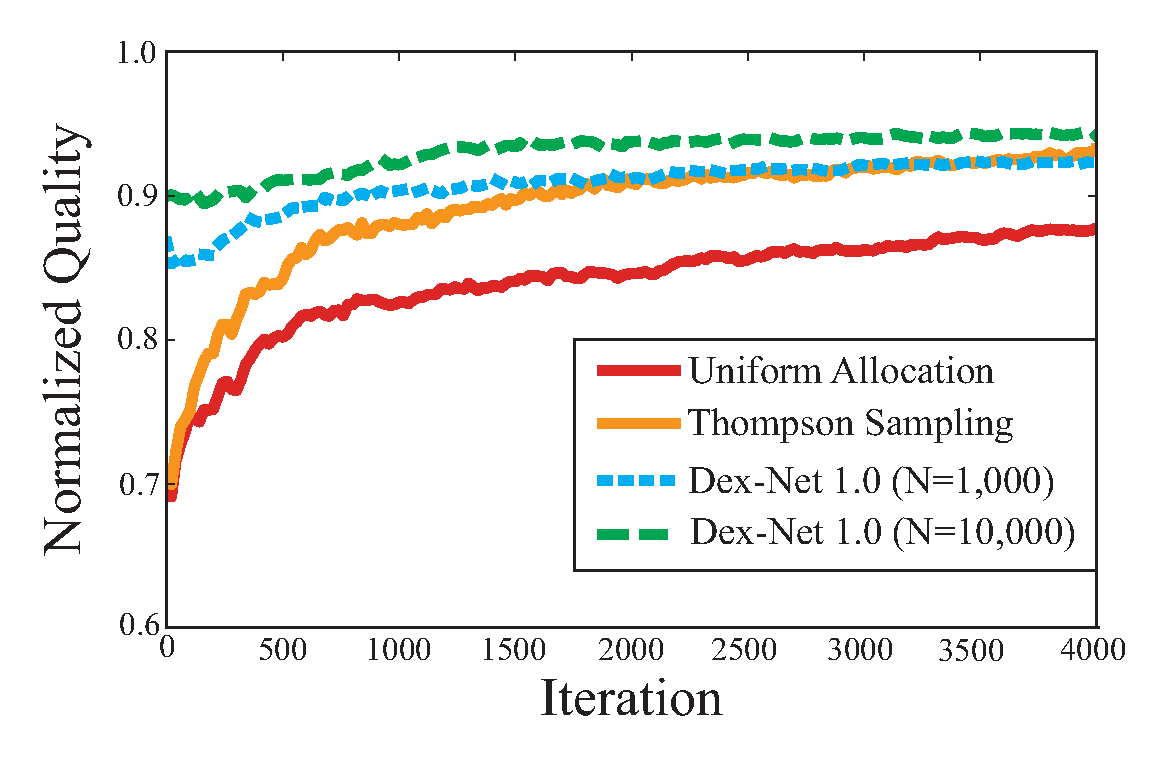
\includegraphics[scale=0.40]{figures/illustrations/avg_reward.eps}
\caption{Average normalized grasp quality versus iteration over 45 test objects and 25 trials per object for the Dex-Net1.0 algorithm with 1,000 and 10,000 prior 3D objects from Dex-Net. We measure quality by the $P_F$ for the best grasp predicted by the algorithm on each iteration and compare with Thompson sampling without priors and uniform allocation. The algorithm converges faster with 10,000 models, never dropping below approximately 90\% of the grasp with highest $P_F$ from a set of 250 candidate grasps.}
\figlabel{avg-reward}
\vspace*{-10pt}
\end{figure}

\subsection{Sensitivity to Object Shape}
\seclabel{shape-sens}
To understand the behavior of the Dex-Net algorithm on individual 3D objects, we examined the convergence rate with a 3D model of a drill and spray bottle from the test set, both uncommon object categories in Dex-Net.
\figref{avg-reward-spray} and  \figref{avg-reward-drill} show the normalized $P_F$ versus iteration averaged over 25 trials for 2,000 iterations on the spray bottle and drill, respectively.
We see that the spray bottle converges very quickly when using a prior dataset of 10,000 objects, finding the optimal grasp in the set in about 1,500 iterations.
This convergence may be explained by the two similar spray bottles retrieved by the MV-CNN from the 10,000 object dataset.
\figref{spray-grasps} illustrates the grasps predicted to have the highest $P_F$ on the spray bottle by the different algorithms after 100 iterations.
On the other hand, performance on the drill does not increase using either 1,000 or 10,000 objects, as the closest model in all of Dex-Net according to the similarity metric is a phone.

\begin{figure}[t!]
\centering
\includegraphics[scale=0.39]{figures/illustrations/drill_avg_reward_w_neighbors.eps}
\caption{Failure object for the Dex-Net 1.0 algorithm. (Top) The drill, which is relatively rare in the dataset, has no geometrically similar neighbors even with 10,000 objects. (Bottom) Plotted is the average normalized grasp quality versus iteration over 25 trials for the Dex-Net 1.0 algorithm with 1,000 and 10,000 prior 3D objects. The lack of similar objects leads to no significant performance increase over Thompson sampling without priors. }
\figlabel{avg-reward-drill}
\vspace*{-10pt}
\end{figure}

\begin{figure}[t!]
\centering
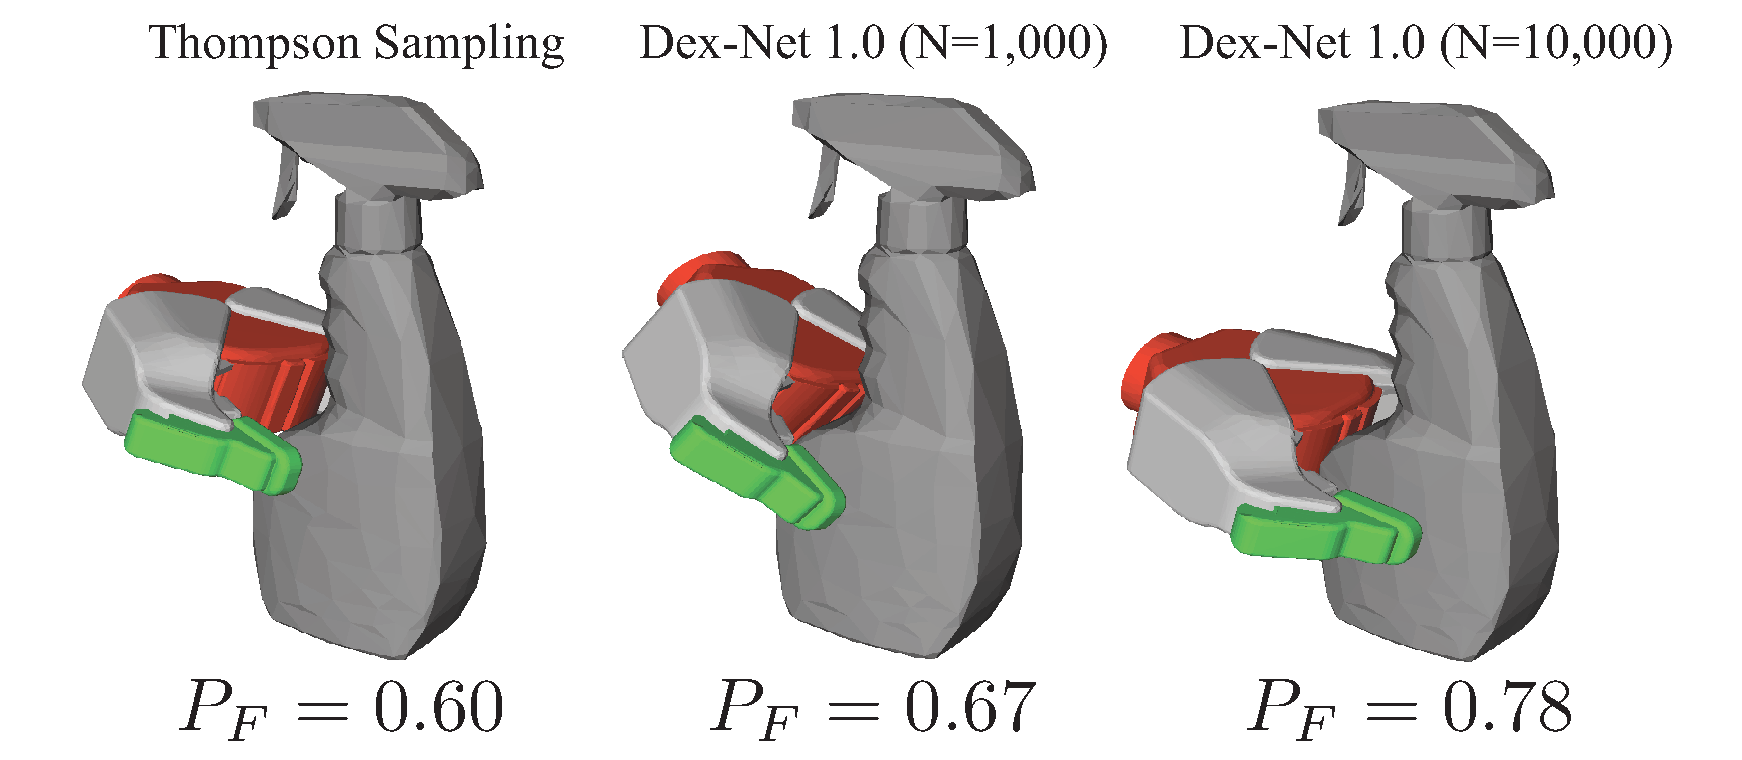
\includegraphics[scale=0.29]{figures/illustrations/spray_grasps.eps}
\caption{Illustration of the grasps predicted to have the highest $P_F$ after only 100 iterations by Thompson sampling without priors and the Dex-Net 1.0 algorithm with 1,000 and 10,000 prior objects. Thompson sampling without priors chooses a grasp near the edge of the object, while the Dex-Net algorithm selects grasps closer to the object center-of-mass.}
\figlabel{spray-grasps}
\vspace*{-5pt}
\end{figure}

\subsection{Sensitivity to Similarity and Uncertainty}
\seclabel{band-sens}
We also studied the sensitivity of the Dex-Net algorithm to the kernel bandwidth hyperparameters described in \secref{ccbps} and the levels of pose and friction uncertainty for the test object.
We varied the inverse bandwidths of the kernel for the grasp parameters and differential heightmaps gradients to the lower values $C_g = diag(0,0,15, 15)$, $\mu_d = 350.0$,  and $\sigma_d = 3.0$ as well as the higher values $C_g = diag(0,0,300, 300)$, $\mu_d = 750.0$,  and $\sigma_d = 1.75$.
We also tested low uncertainty with variances $(\sigma_{t}, \sigma_{r}, \sigma_{\gamma}) = (0.0025, 0.05, 0.05)$ and high uncertainty with variances $(\sigma_{t}, \sigma_{r}, \sigma_{\gamma}) = (0.01, 0.2, 0.2)$ .
\figref{bnu-sens} shows the normalized $P_F$ versus iteration averaged over 25 trials for 2,000 iterations on the 45 test objects.
The results suggest that conservative setting of similiarity kernel bandwidth is important for convergence and that the algorithm is not sensitive to uncertainty levels.

\begin{figure}[t!]
\centering
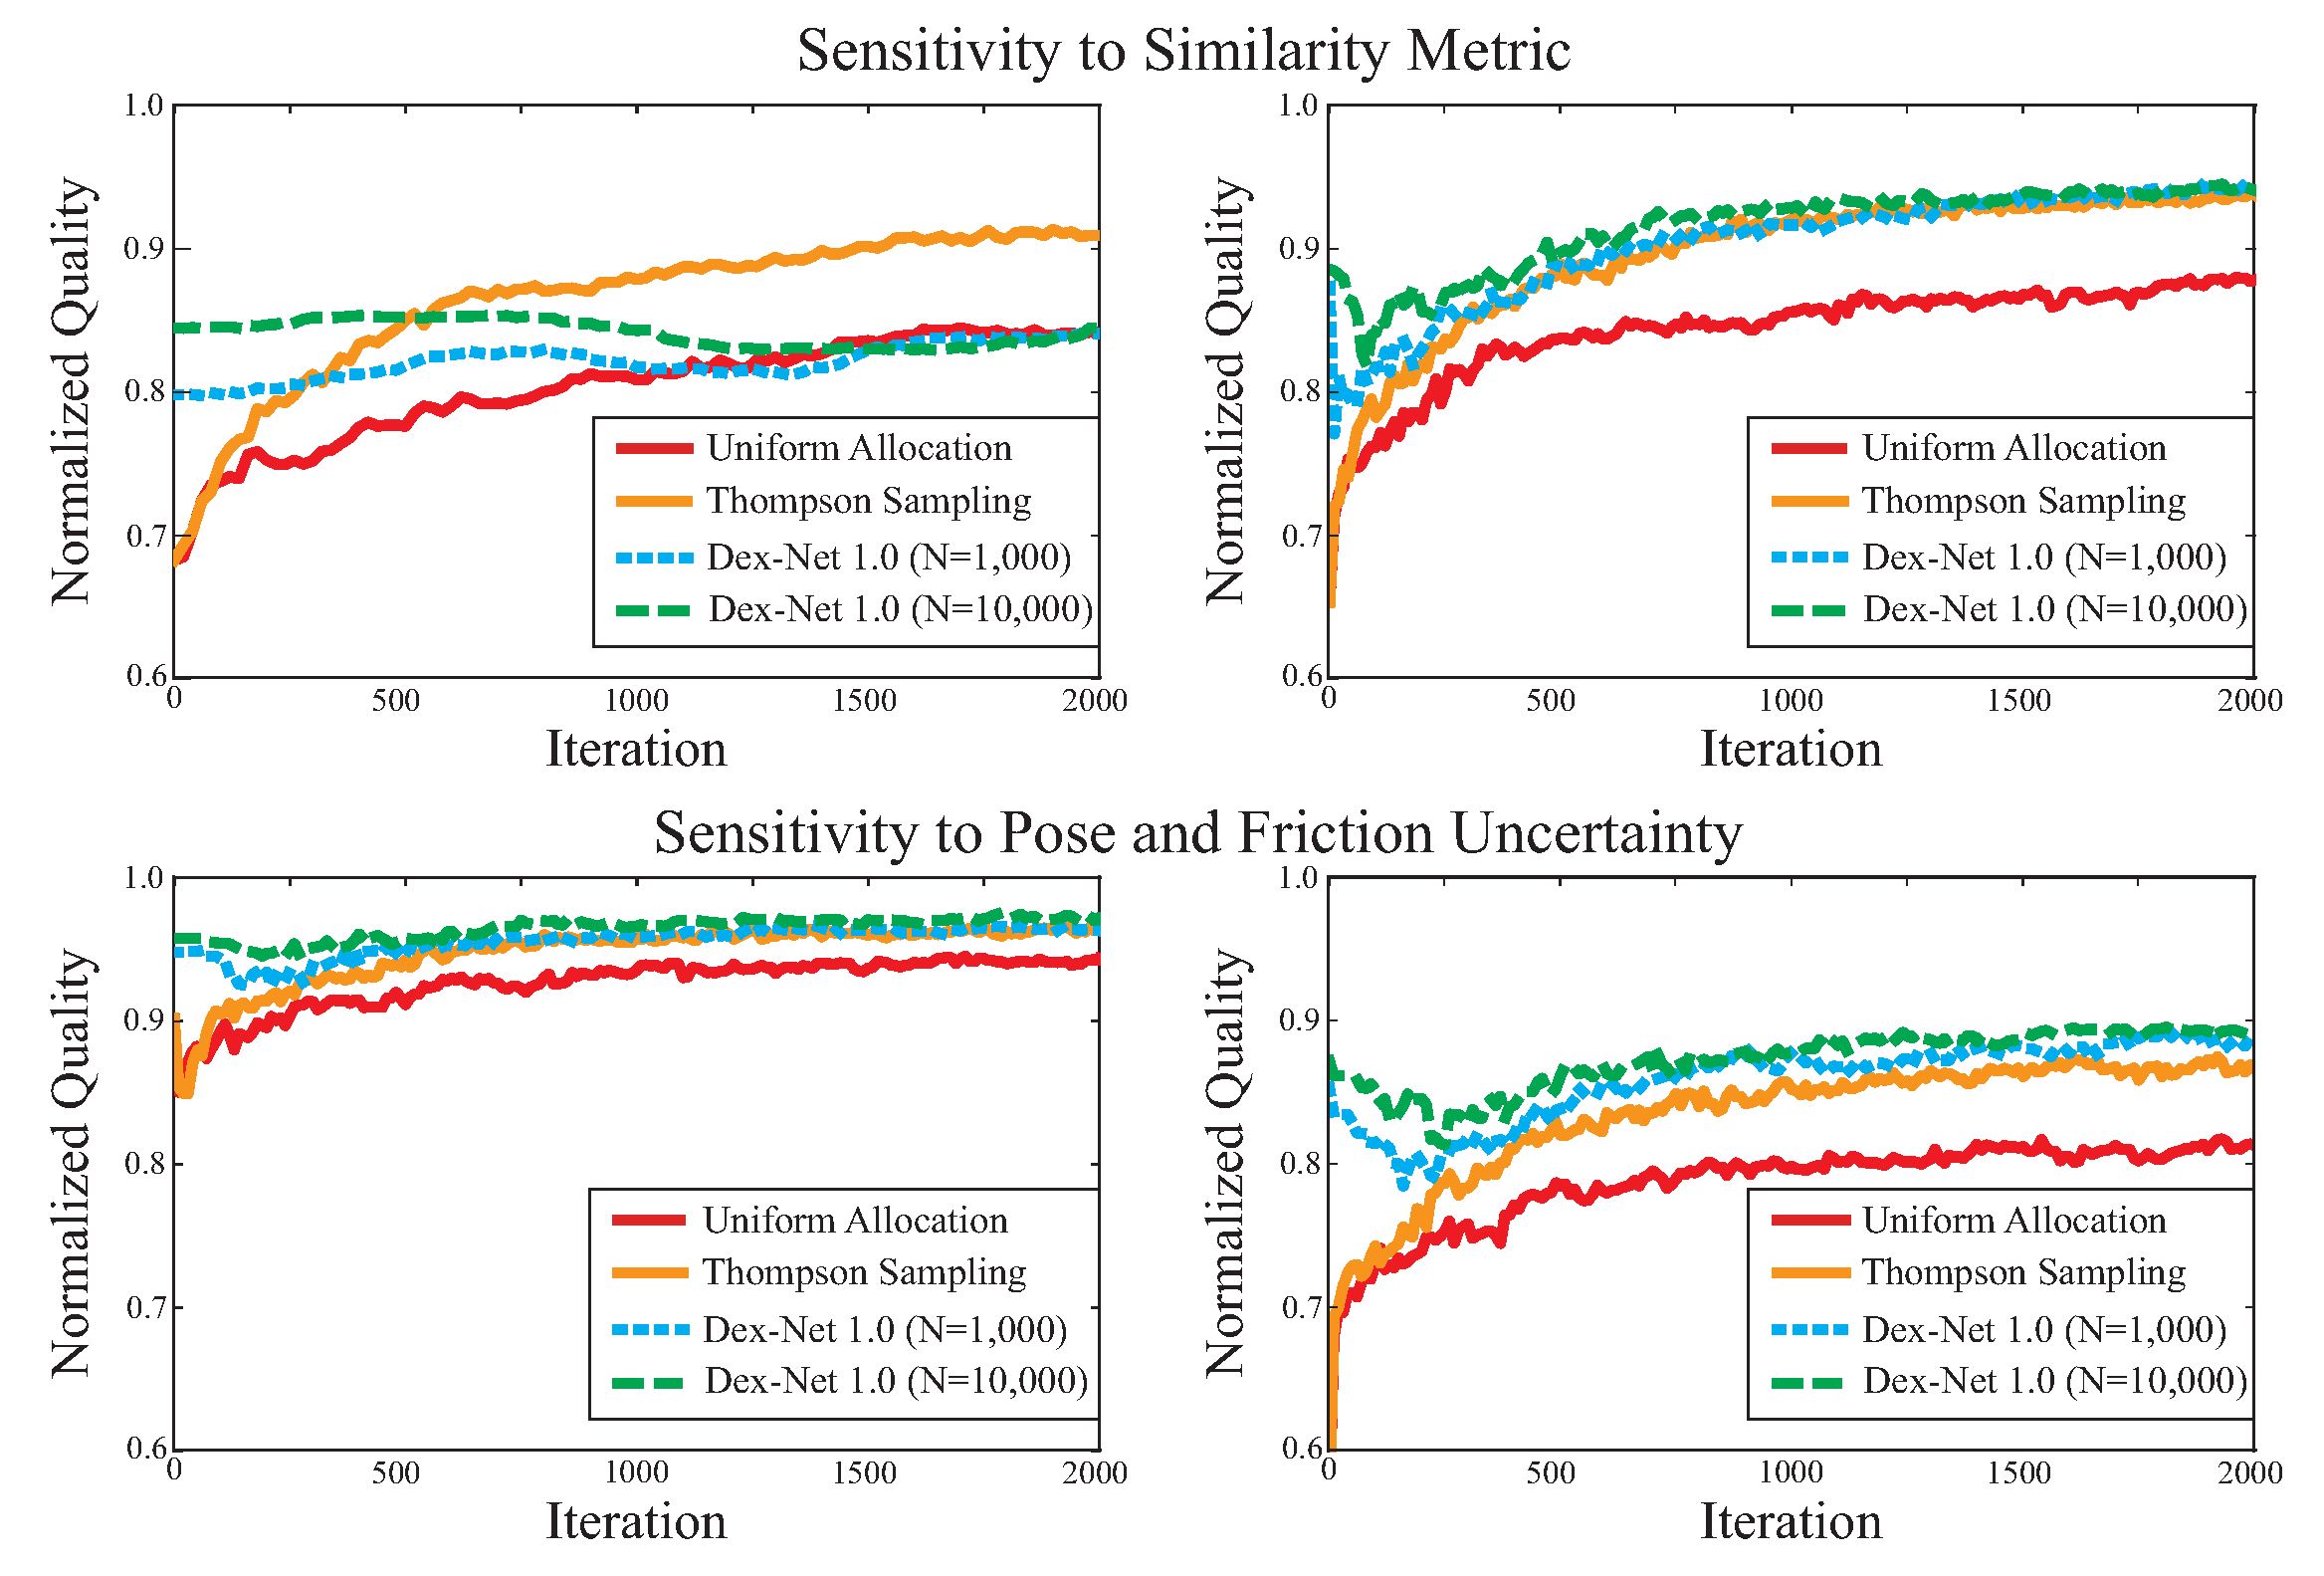
\includegraphics[scale=0.21]{figures/illustrations/combined_weight_and_u_sensitivity.eps}
\caption{Sensitivity to similiarity kernel (top) and pose and friction uncertainty (bottom) for the normalized grasp quality versus iteration averaged over 25 trials per object for the Dex-Net algorithm with 1,000 and 10,000 prior 3D objects.
%with a higher heightmap gradient kernel bandwidth of $1 / 350$ (left) and a lower kernel bandwidth of $1 / 450$ (right).
(Top-left) Using a higher inverse bandwidth causes the algorithm to measure false similarities between grasps, leading to performance on par with uniform allocation.
(Top-right) A lower inverse bandwith decreases the convergence rate, but on average the Dex-Net algorithm still selects a grasp within approximately 85\% of the grasp with highest $P_F$ for all iterations.
(Bottom-left) Lower uncertainty increases the quality for all methods, (bottom-right) higher uncertainty decreases the quality for all methods, and the Dex-Net algorithm with 10,000 prior objects still converges approximately 2$\times$ faster than Thompson sampling without priors. 
}
\figlabel{bnu-sens}
\vspace*{-15pt}
\end{figure}